\documentclass[9pt]{pnas-new}
% Use the lineno option to display guide line numbers if required.
% Note that the use of elements such as single-column equations
% may affect the guide line number alignment. 

% \RequirePackage[english,slovene]{babel} % when writing in slovene
\RequirePackage[slovene,english]{babel} % when writing in english

\usepackage{todonotes}

\templatetype{pnasresearcharticle} % Choose template 
% {pnasresearcharticle} = Template for a two-column research article
% {pnasmathematics} = Template for a one-column mathematics article
% {pnasinvited} = Template for a PNAS invited submission

\selectlanguage{english}
% \selectlanguage{slovene}
% \etal{in sod.} % comment out when writing in english
% \renewcommand{\Authands}{ in } % comment out when writing in english
% \renewcommand{\Authand}{ in } % comment out when writing in english

\newcommand{\set}[1]{\ensuremath{\mathbf{#1}}}
\renewcommand{\vec}[1]{\ensuremath{\mathbf{#1}}}
\newcommand{\uvec}[1]{\ensuremath{\hat{\vec{#1}}}}
\newcommand{\const}[1]{{\ensuremath{\kappa_\mathrm{#1}}}}

\newcommand{\num}[1]{#1}

\graphicspath{{./fig/}}

\title{Collective Behaviour\\ Optimal Shepherding}

% Use letters for affiliations, numbers to show equal authorship (if applicable) and to indicate the corresponding author
\author{Franziska Weber}
\author{Franz Muszarsky}
\author{Kimberley Frings}

\affil{Final Report} 

% Please give the surname of the lead author for the running footer
% \leadauthor{Weber, Muszarsky, Frings} 

% Please add here a significance statement to explain the relevance of your work
% \significancestatement{This is the significance statement.}{add | some | keywords}

% Please include corresponding author, author contribution and author declaration information
%\authorcontributions{Please provide details of author contributions here.}
%\authordeclaration{Please declare any conflict of interest here.}
%\equalauthors{\textsuperscript{1}A.O.(Author One) and A.T. (Author Two) contributed equally to this work (remove if not applicable).}
%\correspondingauthor{\textsuperscript{2}To whom correspondence should be addressed. E-mail: author.two\@email.com}

% Keywords are not mandatory, but authors are strongly encouraged to provide them. If provided, please include two to five keywords, separated by the pipe symbol, e.g:
% \keywords{add | some | keywords} 

\begin{abstract}
Herding denotes a special type of so-called shepherding behaviours in which the shepherds try to steer to flock from a starting point to a target. We investigated the problem of finding optimal herding strategies by building upon an existing agent-based shepherding model. We extended this model by adding a surrounding fence to the environment and by considering the case where multiple shepherds are controlling the flock together. We also implemented an alternative algorithm for multiple shepherds and compared the performance of this algorithm to the one of our model. Our investigations revealed that in most cases the surrounding fence does not influence the shepherding process a lot and that the effect of introducing additional shepherds depends strongly on the behaviour of the flock. 

Our model is publicly available at \url{https://github.com/ki-mberley/Collective-Behaviour}.
\end{abstract}

\dates{\textbf{\today}}
\program{BM-RI}
\vol{2023/24}
\no{CB:GA} % group ID
%\fraca{FRIteza/201516.130}

\begin{document}

% Optional adjustment to line up main text (after abstract) of first page with line numbers, when using both lineno and twocolumn options.
% You should only change this length when you've finalised the article contents.
\verticaladjustment{-2pt}

\maketitle
\thispagestyle{firststyle}
\ifthenelse{\boolean{shortarticle}}{\ifthenelse{\boolean{singlecolumn}}{\abscontentformatted}{\abscontent}}{}

% If your first paragraph (i.e. with the \dropcap) contains a list environment (quote, quotation, theorem, definition, enumerate, itemize...), the line after the list may have some extra indentation. If this is the case, add \parshape=0 to the end of the list environment.
\textit{Shepherding behaviors} are a class of flocking behaviors in which one or more agents (called \textit{shepherds}) try to control the motion of another group of agents (called \textit{flock}) by exerting repulsive forces. A real-life example are sheep dogs guiding flocks of sheep. \textit{Herding} denotes a special type of shepherding behavior in which the shepherds attempt to steer the flock from a starting point to a target. \cite{lien2003shepherding}

In the context of the course \textit{Collective Behavior}, we decided to investigate the problem of finding optimal herding strategies. To begin our work, we have chosen the paper titled \textit{Optimal Shepherding and Transport of a Flock} \cite{ranganathan2022optimal} by A. Ranganathan, A. Heyde, A. Gupta, and L. Mahadevan as a starting point. This paper models herding as an optimization problem for the shepherd using an agent-based approach.

This initial report provides an overview of the present state of our project. We start by giving a concise summary of the relevant parts of our selected paper, followed by a description of our steps involved in executing the existing agent-based model (ABM). Subsequently, we present the current state of our GitHub-Repository and describe our strategy and our goals for the further course of this project.


\section*{Methods}
\subsection{Description of the original model}

The herd consists of $N$ agents which move in a two-dimensional open field. The behaviour of the agents is based on Reynolds' boids model \cite{boids}. To be more precise, the movement of each agent depends on three agent-agent interactions, namely local alignment, repulsion, and weak attraction to the herd center, and on the repulsion from the shepherd.

This leads to the following velocity field of an agent in the herd, where $\alpha, \beta, \gamma$, and $\delta$ are weights:

\begin{equation}
\label{eq:agent_velocity}
\boldsymbol{v}^{\text{net}} = \alpha \boldsymbol{v}^{\text{alignment}}_{a-a} + \beta \boldsymbol{v}^{\text{repulsion}}_{a-a} + \gamma \boldsymbol{v}^{\text{attraction}}_{a-a} + \delta \boldsymbol{v}^{\text{repulsion}}_{a-s} 
\end{equation}

Local alignment means that agents that are close to each other align their velocity vectors. We use the formulation from the Vicsek model \cite{alignment}: At each timestep, the orientation of agent $i$ is updated to be the sum of the average $\langle \theta \rangle$ of the orientations of the other agents within a certain interaction radius $r^\text{alignment}$ and a uniformly distributed noise $\eta \in [-\eta_0 / 2, \eta_0 / 2]$, i.e., $\theta^\text{alignment}(i) = \langle \theta \rangle_{r < r^\text{alignment}} + \eta$. $r^\text{alignment}$ is set to approximately ten times the agent size $l_a$. The local alignment term of agent $i$ arises as the orientation of this agent multiplied by the agent speed $v_a$:

$$\boldsymbol{v}^{\text{alignment}}_{a-a}(i) = v_a 
 \left(\cos \theta^\text{alignment}(i), \sin\theta^\text{alignment}(i)\right)$$

The repulsion between the agents is modeled as
$$\boldsymbol{v}^{\text{repulsion}}_{a-a}(i) = \sum_{i \neq j} \exp\left( -\frac{\Vert\boldsymbol{r_{ji}}\Vert}{l_a}\right)\frac{\boldsymbol{r_{ji}}}{\Vert\boldsymbol{r_{ji}}\Vert}$$
with $\boldsymbol{r_{ji}} = \boldsymbol{r_i} - \boldsymbol{r_j}$ where $r_k$ denotes the position of agent $k$.

The attraction to the herd center quantifies the idea that agents intend to move to the middle of the herd to avoid being captured by predators. In our model, the attraction term is independent of an agent's distance to the herd center but only depends on the agents' speed and the polar angle $\phi(i) = \tan^{-1}\left(\frac{y_\text{cm} - y_i}{x_\text{cm} - x_i}\right)$ between the agent's position $(x_i, y_i)$ and the herd's center of mass $\boldsymbol{r_\text{cm}} = (x_\text{cm}, y_\text{cm})$:
$$\boldsymbol{v}^\text{attraction}_{a-a}(i) = v_a \left(\cos \phi(i), \sin \phi(i)\right)$$

Lastly, the repulsion of an agent from the shepherd is modeled similarly to the repulsion between two agents:

$$\boldsymbol{v}^\text{repulsion}_{a-s}(i) = \exp\left(\frac{-\Vert\boldsymbol{r_{si}}\Vert}{l_s}\right)\frac{\boldsymbol{r_{si}}}{\Vert\boldsymbol{r_{si}}\Vert}$$
with $\boldsymbol{r_{si}}=\boldsymbol{r_i} - \boldsymbol{r_s}$ where $\boldsymbol{r}_s$ is the position of the shepherd and $\boldsymbol{r}_i$ is the position of agent $i$. Based on observations of real-world shepherds, $l_s$ was chosen as approximately 30 times $l_a$.

The behaviour of the shepherd is not predefined but arises from its goal to transport the entire herd to a certain target position. This goal leads to three conditions, namely $(A)$ the shepherd should move the herd's center of mass to the target, $(B)$ the shepherd may not lose any agents in the process, and $(C)$ the shepherd should keep target and herd in alignment to maintain the line of sight.

These three transport requirements are weighted with $W_\text{mean}, W_\text{std}$ and $W_\text{col}$ respectively and linearly combined into an objective function for the shepherd:
\begin{equation}
\label{eq:objective_function}
    C(\boldsymbol{r_s}) = W_\text{mean}|\boldsymbol{\Delta r}| + W_\text{std} \sigma_{r_\text{cm}} + W_\text{col} |\boldsymbol{\Delta R}_\text{col}|
\end{equation}

The importance of transporting the herd to the target is represented by $|\boldsymbol{\Delta r}| = |\boldsymbol{r}_\text{target} - r_\text{cm}|$, where $\boldsymbol{r}_\text{target}$ is the position of the target. $\sigma_{r_\text{cm}} = \left(\frac{\sum_i(r_i - r_\text{cm})^4}{N}\right)^{1/4}$ models the objective of keeping the herd cohesive and not losing any agents. The advantage gained from keeping the flock within the line of sight of the shepherd is represented by $\boldsymbol{\Delta R_\text{col}} = \boldsymbol{r_s} + l_s \frac{\boldsymbol{r_\text{cm - target}}}{\Vert \boldsymbol{r_\text{cm - target}} \Vert}$ where $\boldsymbol{r_\text{cm - target}} = \boldsymbol{r_\text{target}} - \boldsymbol{r_\text{cm}}$.

The actual simulation is based on a forward Euler scheme implemented in C++. At each timestep, the positions of all agents are updated based on formula \ref{eq:agent_velocity}. For the shepherd, several directions are randomly sampled from the uniform distribution on $[0, 2\pi)$ and the direction corresponding to the minimal value of the objective function is chosen. 

\subsection{Implementation of the surrounding fence}
The original implementation provided by the paper's authors included a code base featuring a fence implementation, specifically a function for calculating the repulsion force exerted by a fence on a sheep. However, due to the lack of explanation in the paper regarding the interpretation of the fence and the difficulty of understanding the author's implementation solely through code inspection, we decided not to use their code. Instead, we opted for a basic fence implementation, leaving room for potential future extensions such as incorporating an actual repulsion force from the fence.

We introduced minimum and maximum $x$- and $y$-coordinates, defining the boundaries of the surrounding fence. When calculating the next step for a sheep or dog, if the computed value exceeds the established fence bounds, we adjust the next step's value to the corresponding minimum or maximum $x$- or $y$-coordinate, preventing the sheep or dog from crossing the fence. This modification was integrated into the parameters file (\texttt{params.txt}) to accommodate fence specifications as input. Additionally, we included a condition in the \texttt{timestepping.hh} file to update the next step in the presence of a fence. As a final step, we ensure that a fence is shown in the plot by incorporating the necessary code in \texttt{trajectory\_plotter.py} and \texttt{visualizer.py}.

\subsection{Implementation of multiple shepherds}
We began our study by exploring existing literature that showcased the use of multiple dogs for shepherding \cite{kubo2022herd}, \cite{baxter2021simulating}. Through this research, we found that in order to adapt the model for multiple shepherds, we needed to make two modifications. Firstly, we aimed to include a mechanism that discourages shepherds from getting too close to each other. Secondly, we wanted to adjust the way sheep and shepherds repel each other, ensuring it considered the sum of the repulsions between sheep and each individual shepherd. Although the latter was already part of the original paper's implementation, it was not functioning correctly, and we corrected the code to ensure its proper operation.

To prevent the shepherds from coming too close to each other, we added an additional term to the cost function which models the proximity of one shepherd to the other ones. We defined the proximity as the inverse of the distance, so two shepherds that are very close to one another are penalized more heavily. The proximity penalty for one shepherd is the sum of the proximities of all other shepherds. We introduced a parameter named \texttt{shepherd\_distance\_penalty} which is used to balance the proximity penalty with the other terms in the cost function.

With these adjustments in place, we successfully implemented a basic version of the model with multiple shepherds.

\subsection{Implementation of an agent-based shepherding model as a basis for comparison}

To test whether our implementation and especially our extensions of the model were working well, we wanted to compare its performance to the one of an algorithm from the literature. During our research on existing multiple-shepherd algorithms, we determined the agent-based model from the paper \textit{Simulating Single and Multiple Sheepdogs Guidance of a Sheep Swarm} \cite{baxter2021simulating} to be the most suitable for our purposes.

In this paper, the shepherds are modeled as agents that act based on the goals of keeping the herd cohesive and guiding it towards the target. Additionally, each shepherd is at the same time attracted to the center of mass of the other shepherds and repelled from other shepherds if they are coming too close.

Because the paper did not provide an implementation, we recreated a basic version of the algorithm ourselves. As the sheep model in \cite{baxter2021simulating} is very similar to the sheep model from our chosen paper \cite{ranganathan2022optimal}, we reused our existing sheep model and only adapted the model of the shepherd.

\section*{Results}
\label{sec:results}
\subsection{Results when introducing second shepherd}
The implementation of a second shepherd introduces an additional dog whose task is the guide the sheep towards the target. Figures \ref{fig:single-shepherd} and \ref{fig:second-shepherds} illustrate the results for trajectories with one and two shepherds. A distance penalty of 0.05 was applied. As planned, the introduction of a second shepherd is evident, and it appears to follow a trajectory similar to that of the initial shepherd but at a higher speed. Further evaluation is needed to determine whether this is always the case.

\begin{figure}[!h]
    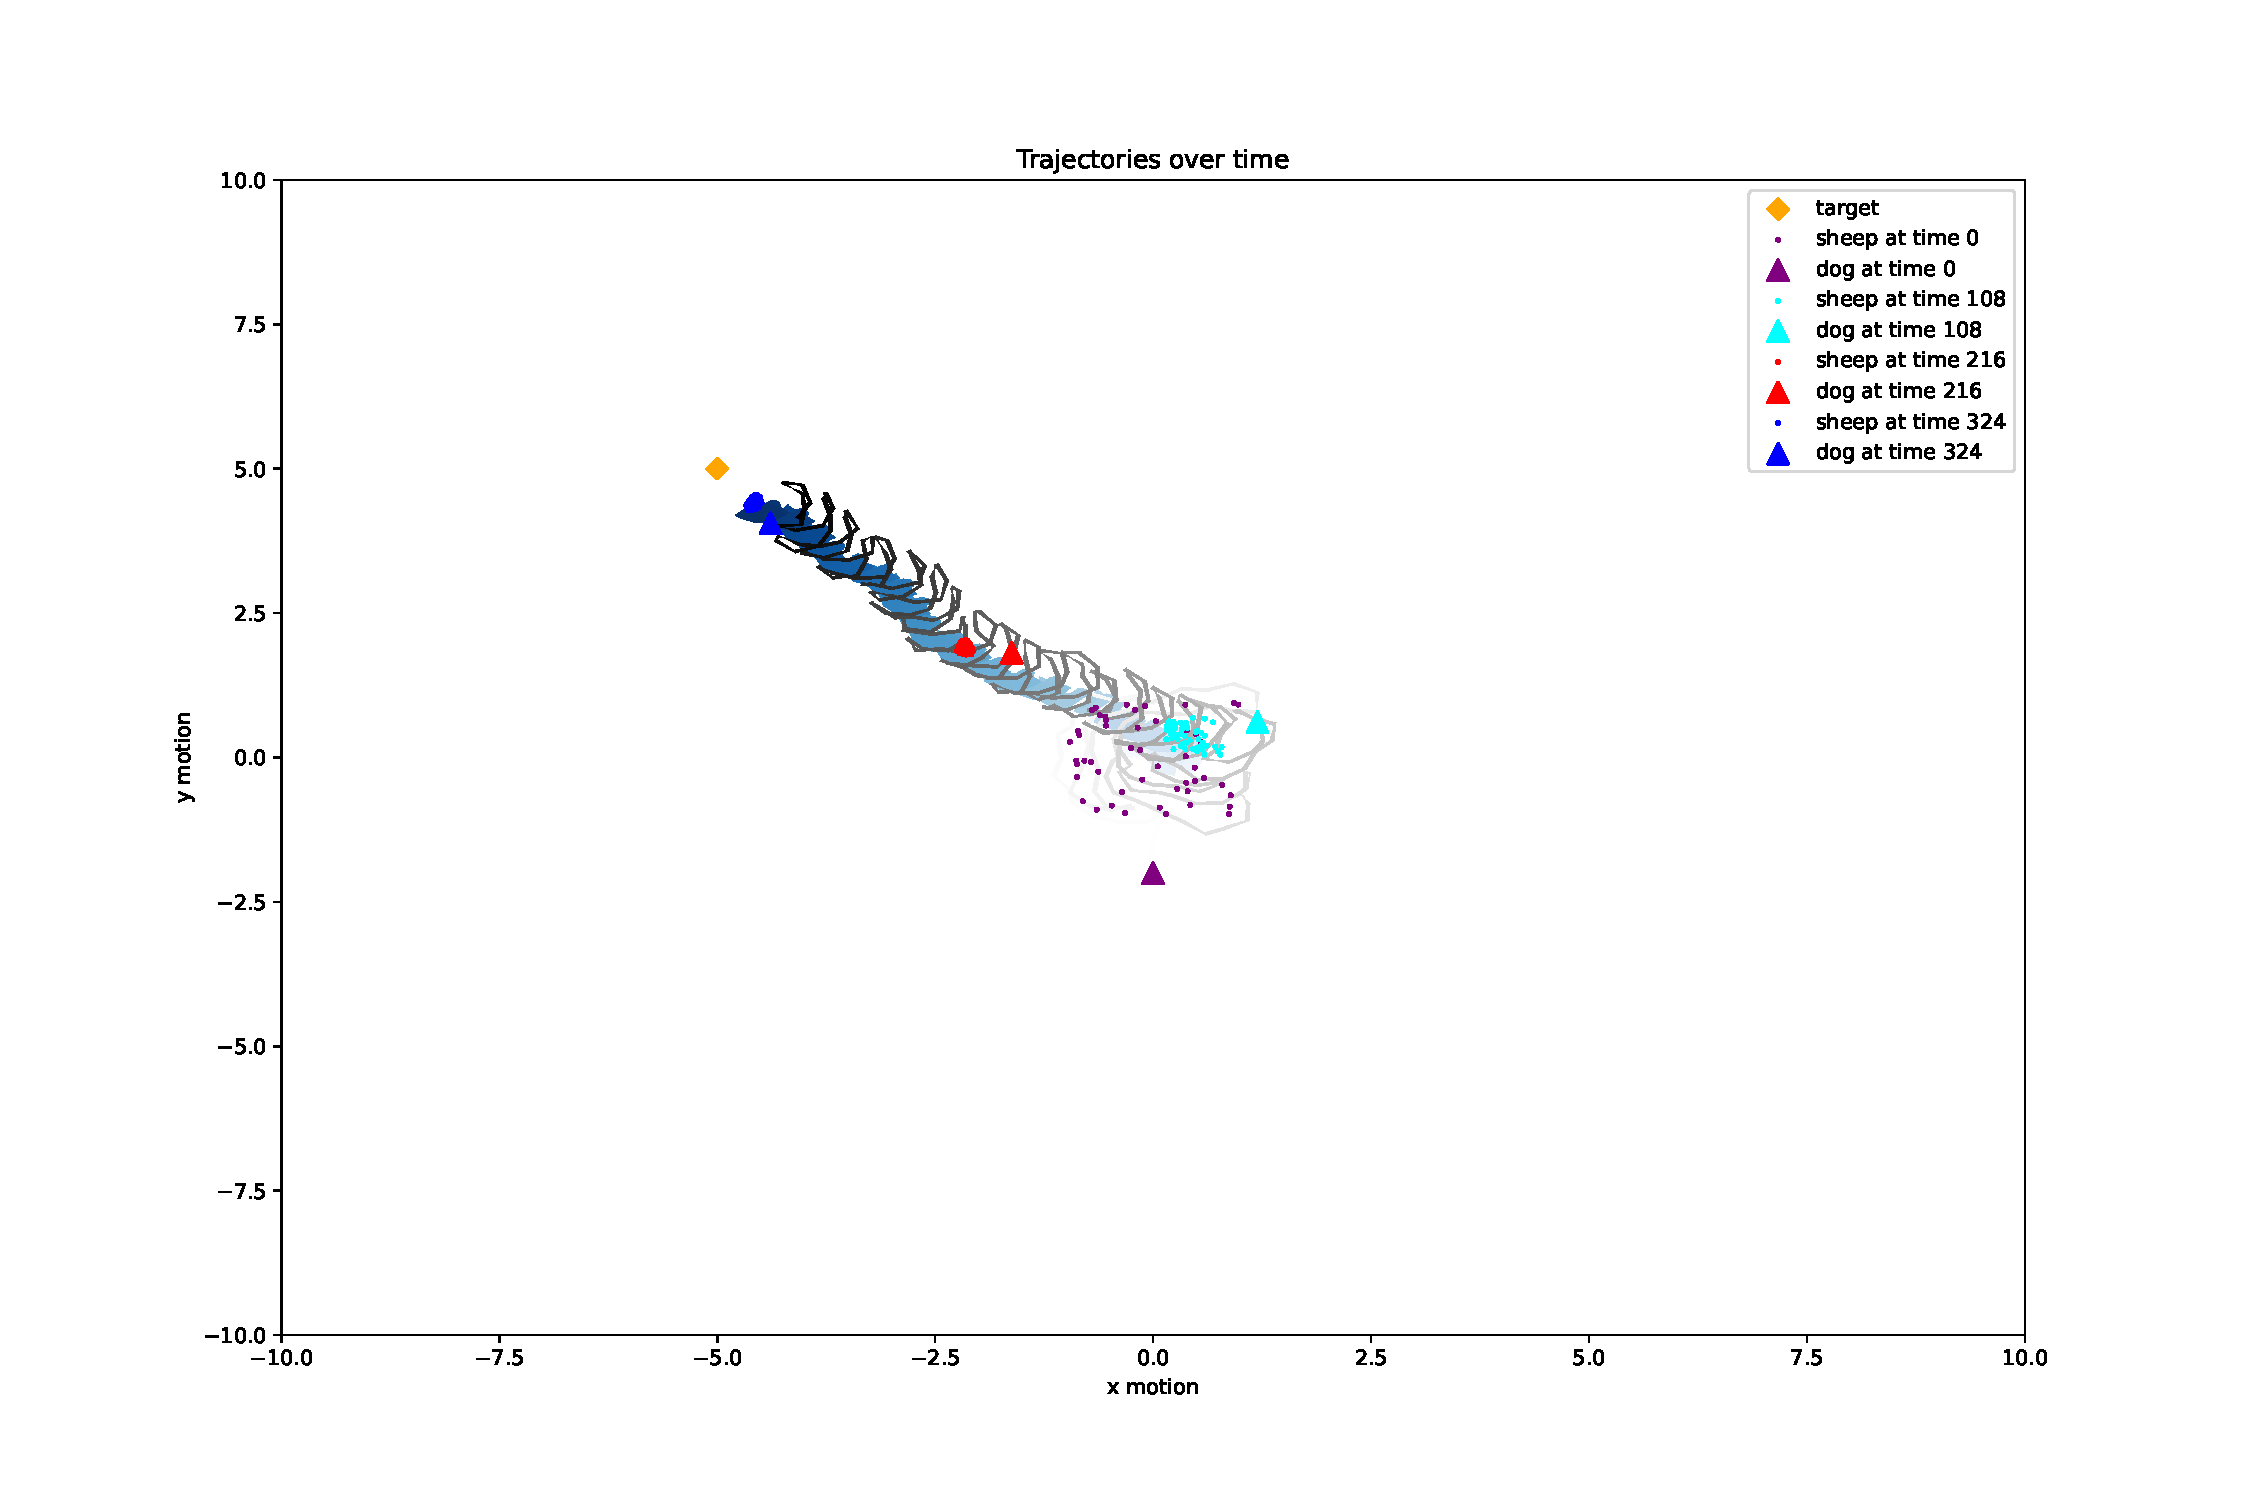
\includegraphics[width=0.9\textwidth]{figures/single-shepherd.pdf}
    \caption{Trajectory plot using a single shepherd}
    \label{fig:single-shepherd}
\end{figure}

\begin{figure}[!h]
    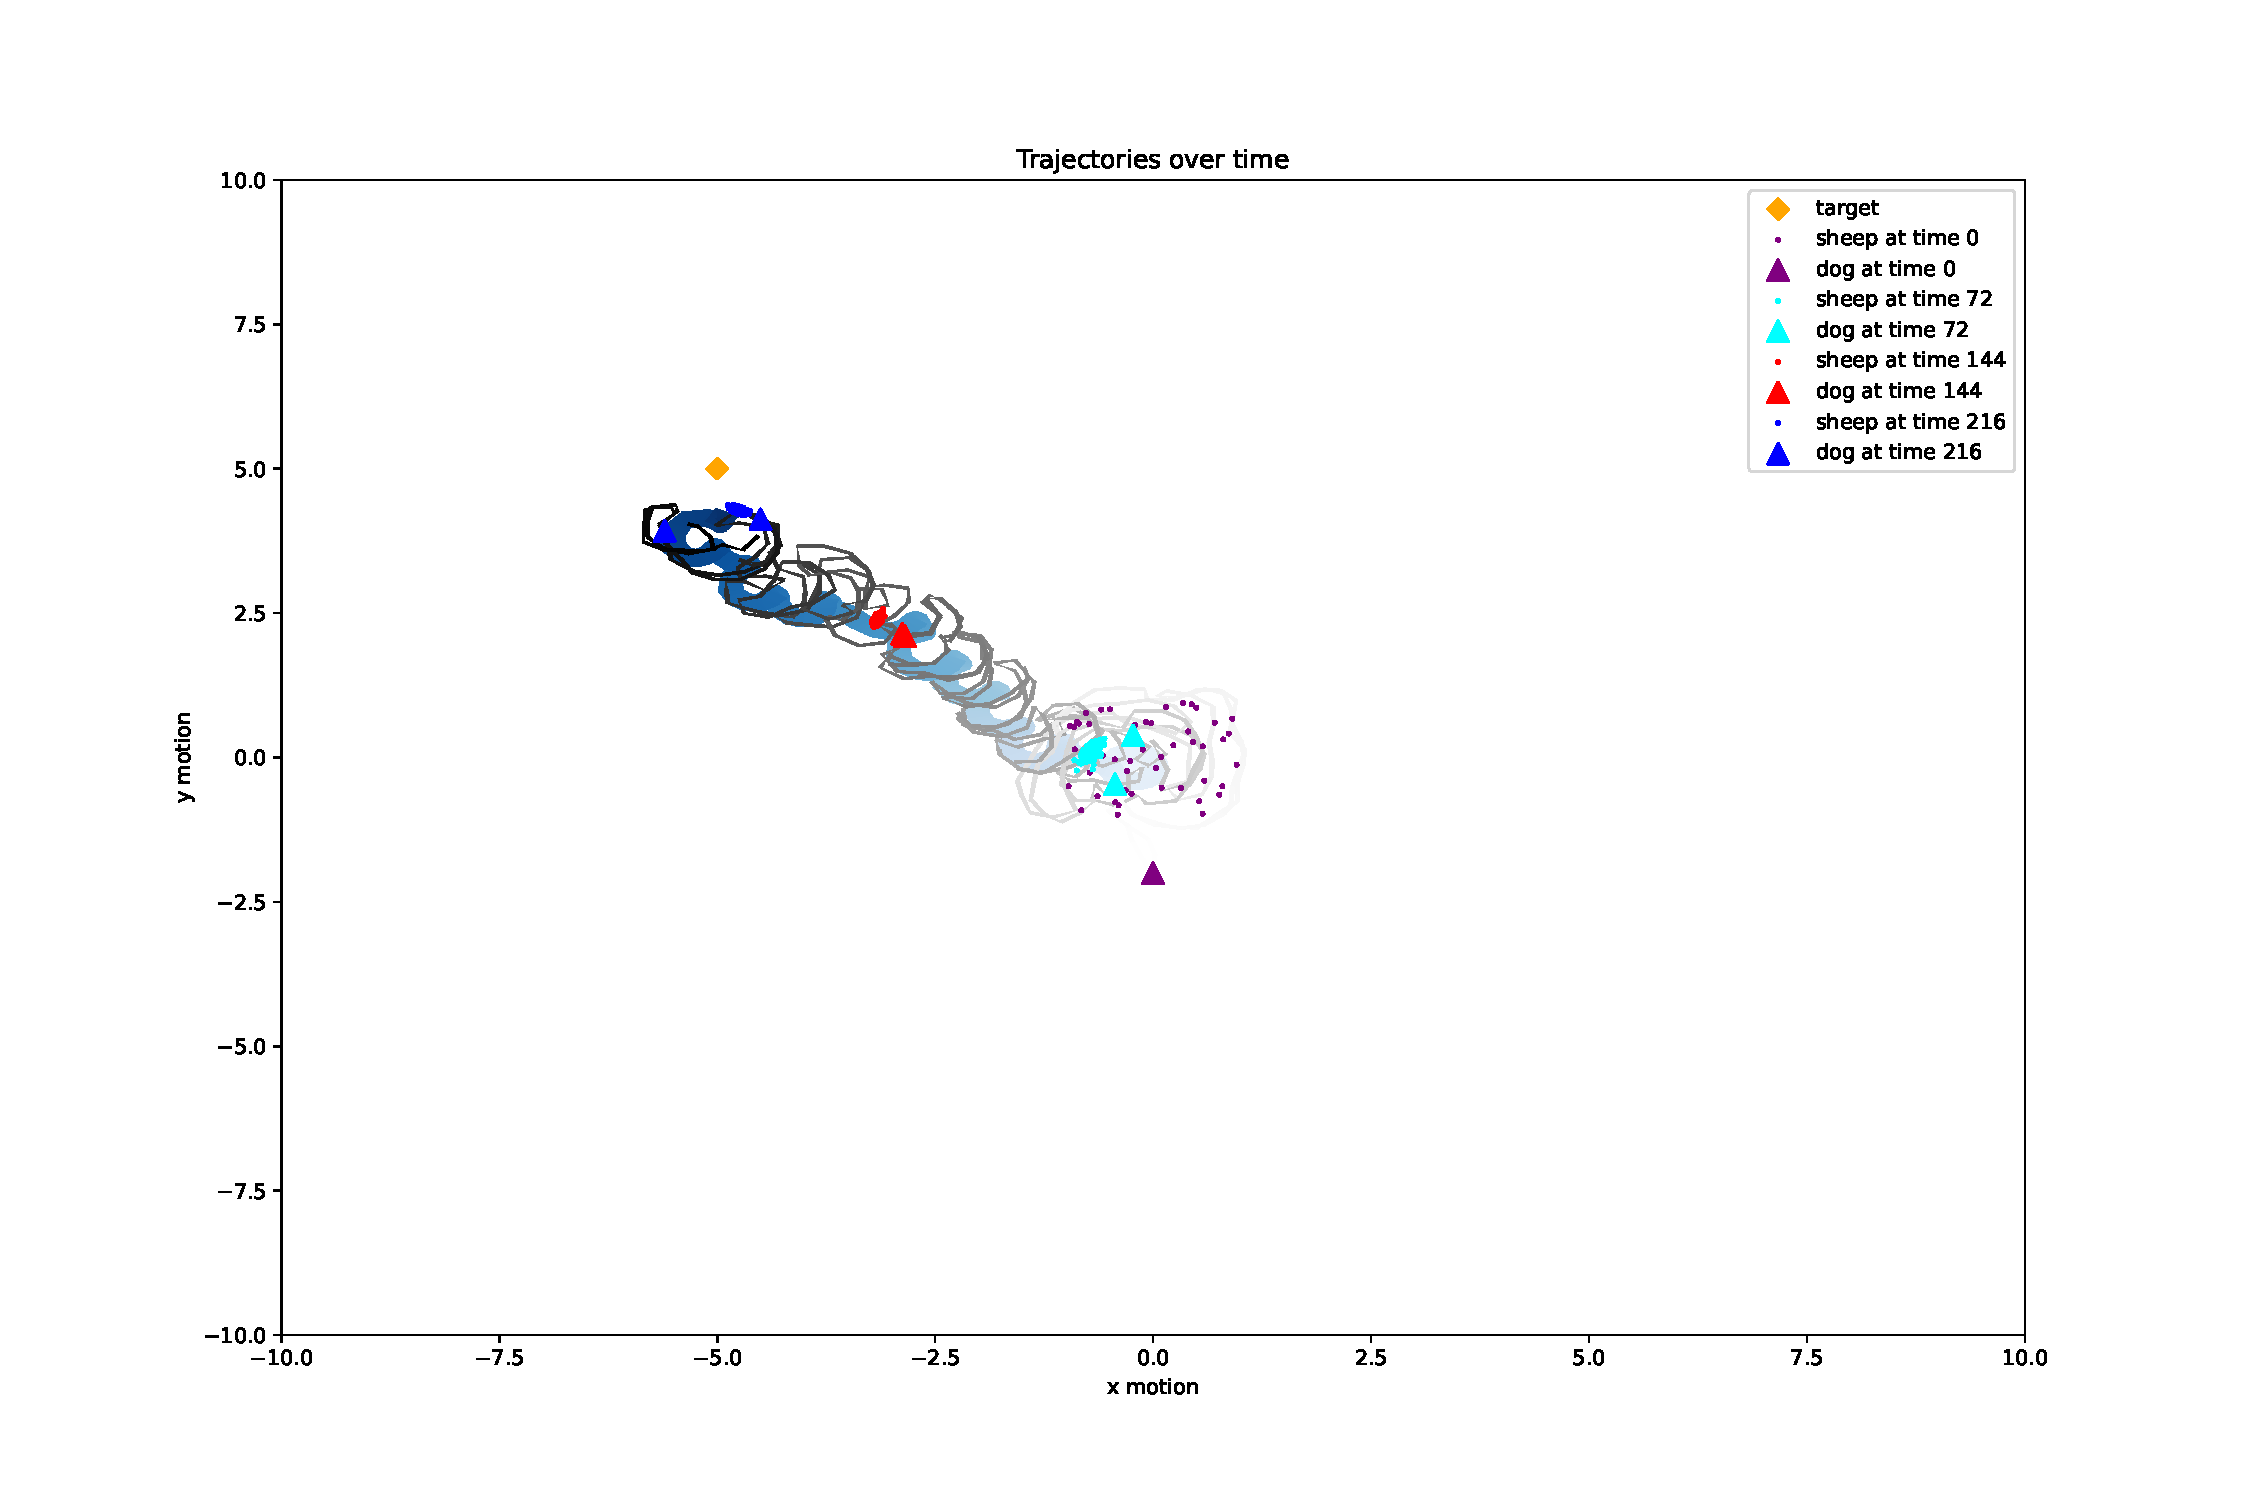
\includegraphics[width=0.9\textwidth]{figures/second-shepherd.pdf}
    \caption{Trajectory plot using two shepherds}
    \label{fig:second-shepherds}
\end{figure}

\newpage


\subsection{Results when introducing a fence}
%%%% TODO: position correctly when all other text has also been added
The implementation of a fence ensures that both the dogs and sheep are surrounded by a boundary and prevents them from crossing it. In the figures below, the outcomes are depicted for the herding style 'driving' with and without a fence. As intended, the presence of the fence effectively confines the sheep and dogs within its boundaries, while the dog still leads the sheep to the target.

\begin{figure}[!h]
    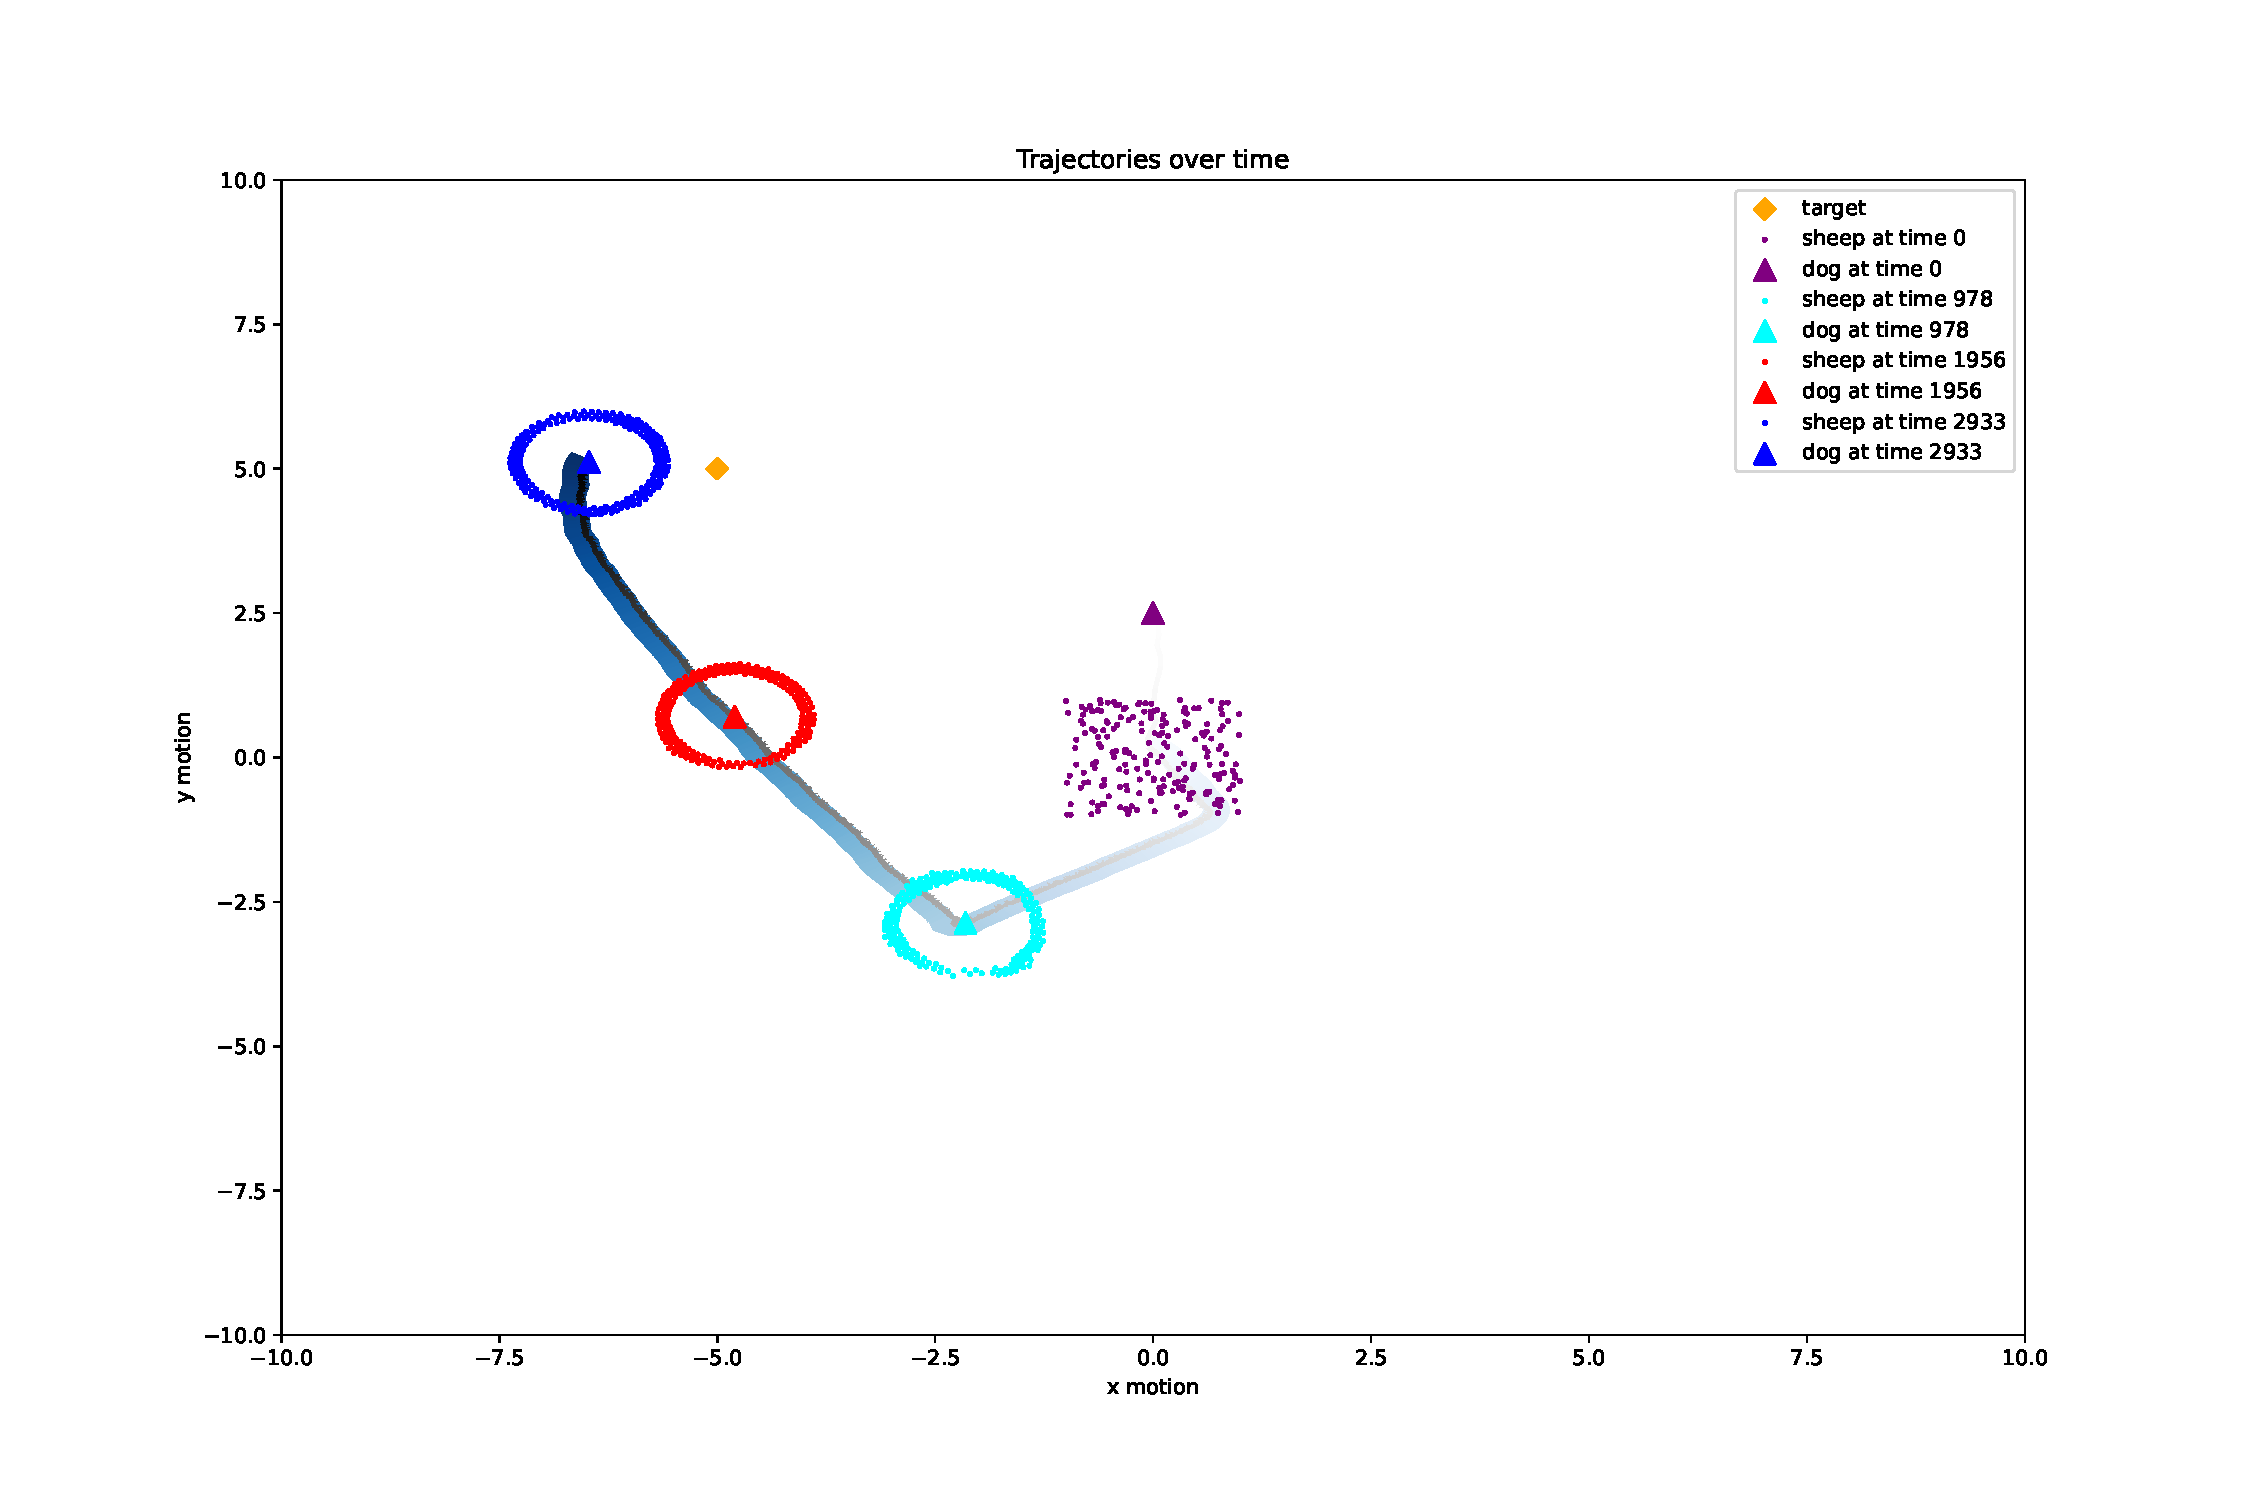
\includegraphics[width=0.9\textwidth]{figures/driving.pdf}
    \caption{Trajectory plot for driving without a fence}
\end{figure}

\begin{figure}[!h]
    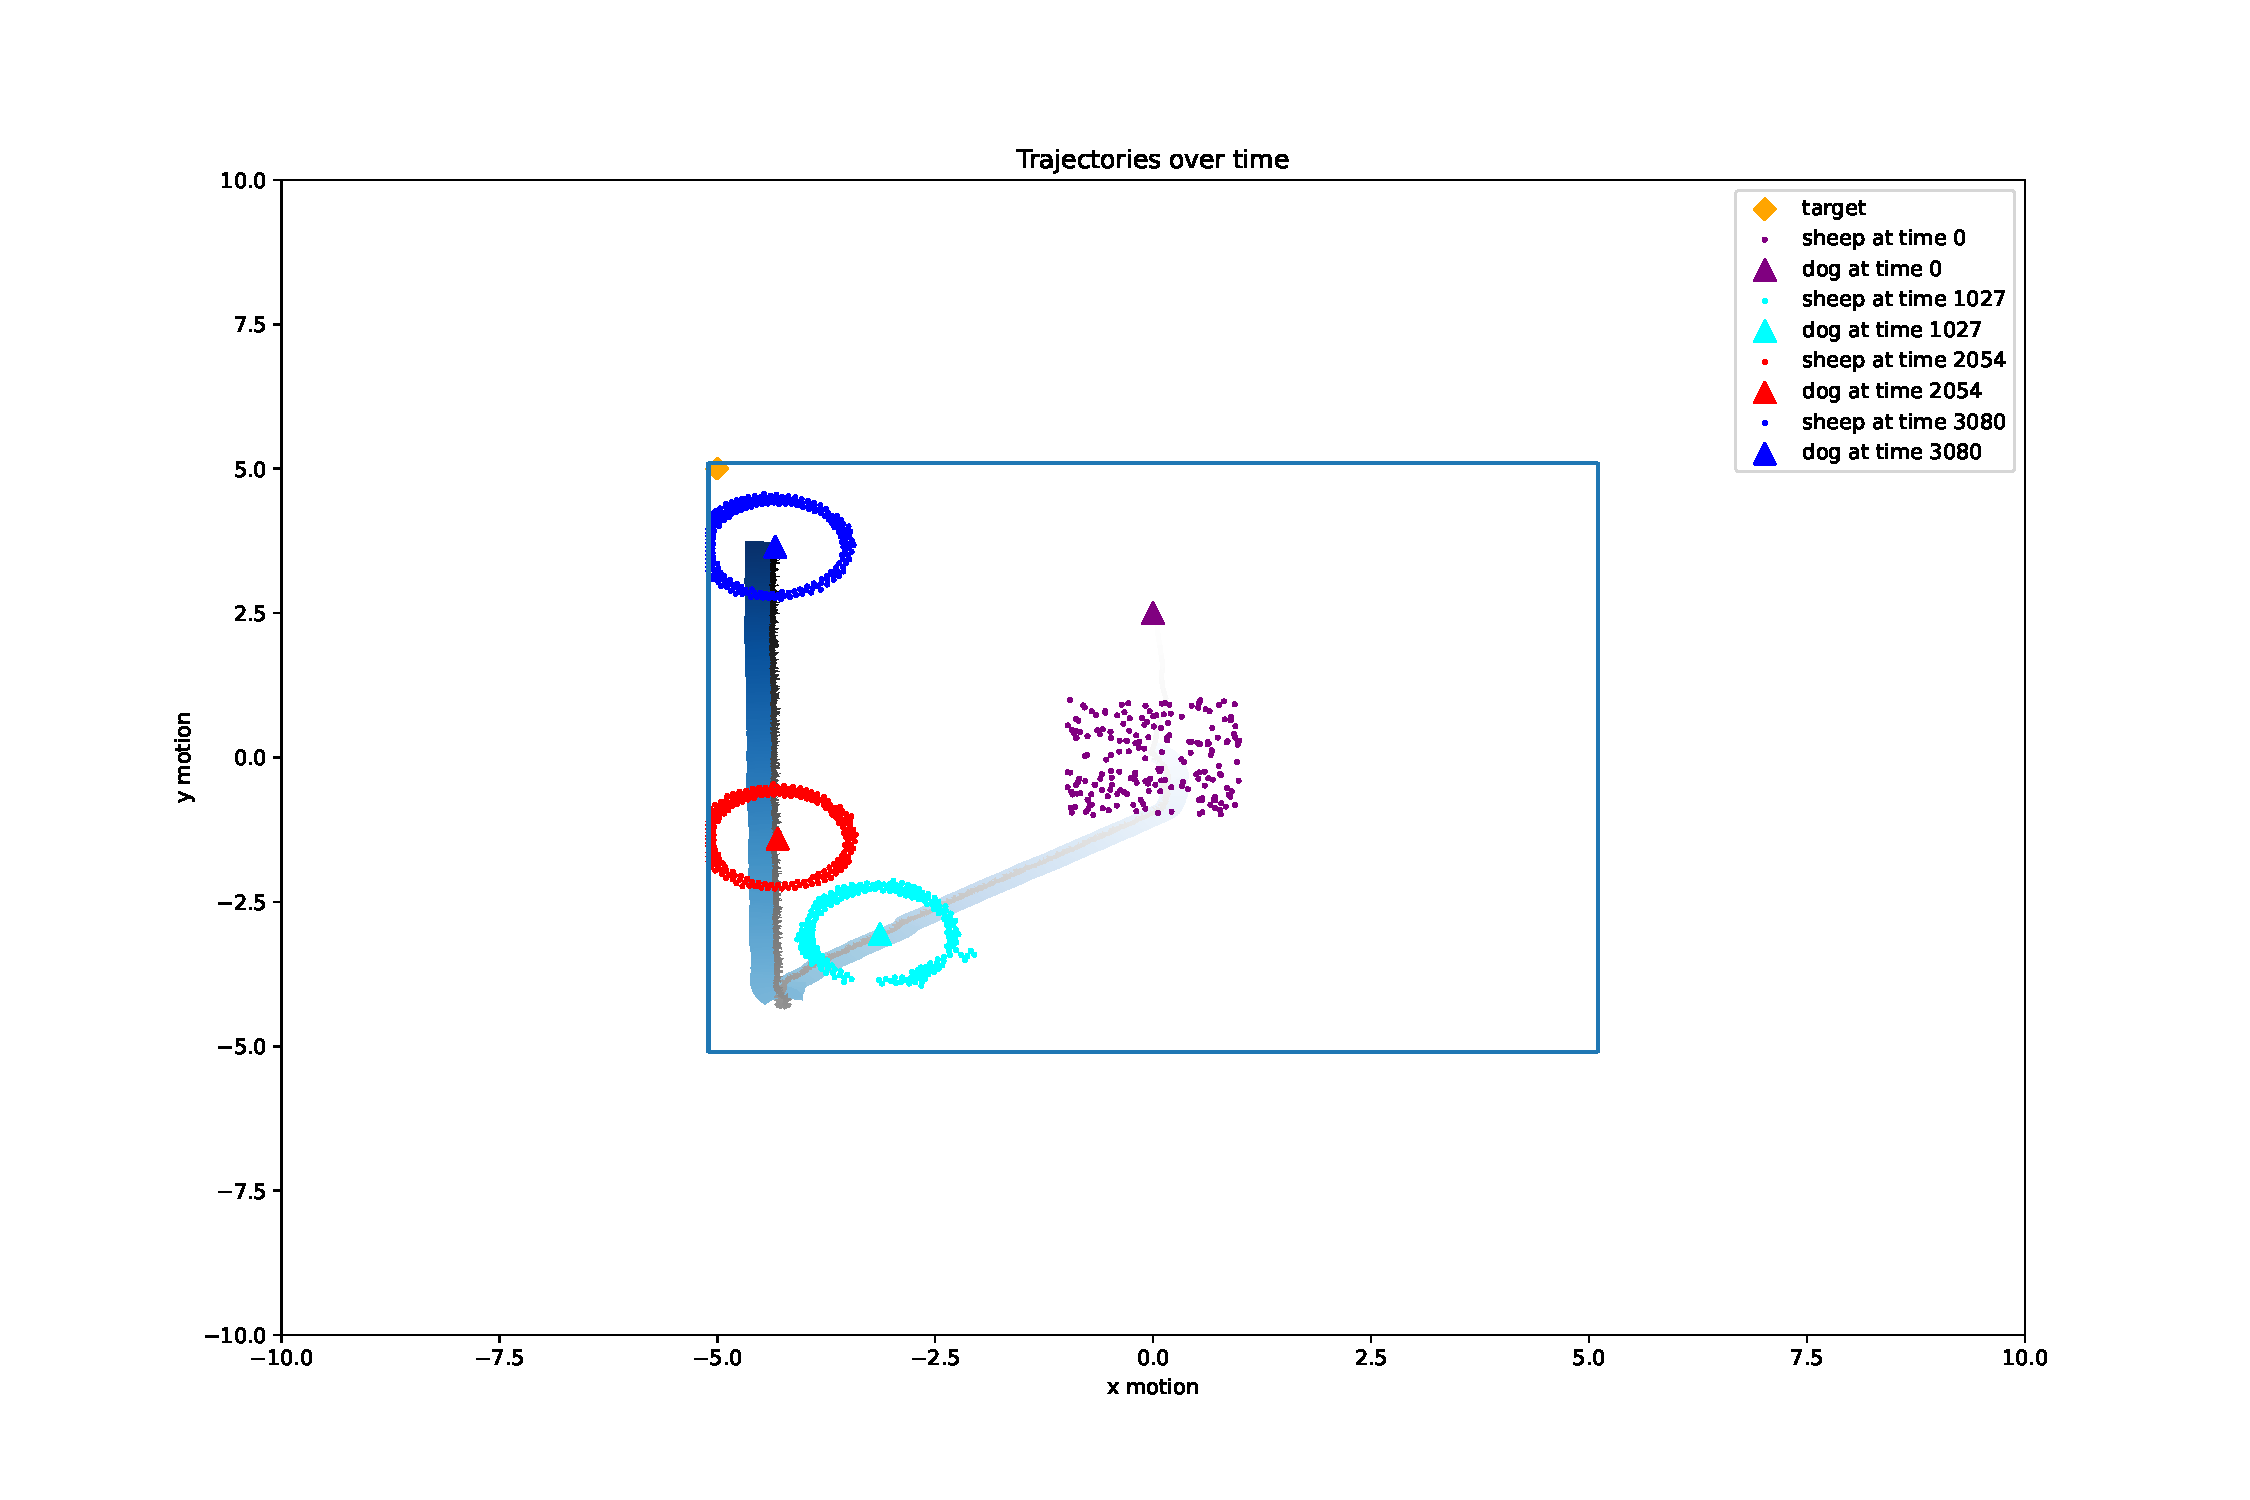
\includegraphics[width=0.9\textwidth]{figures/driving-fence.pdf}
    \caption{Trajectory plot for driving with a fence}
\end{figure}

\newpage


%%% TODO: either include in appendix or leave out
% \begin{figure}[!h]
%   \centering
%   \begin{minipage}[b]{0.49\textwidth}
%     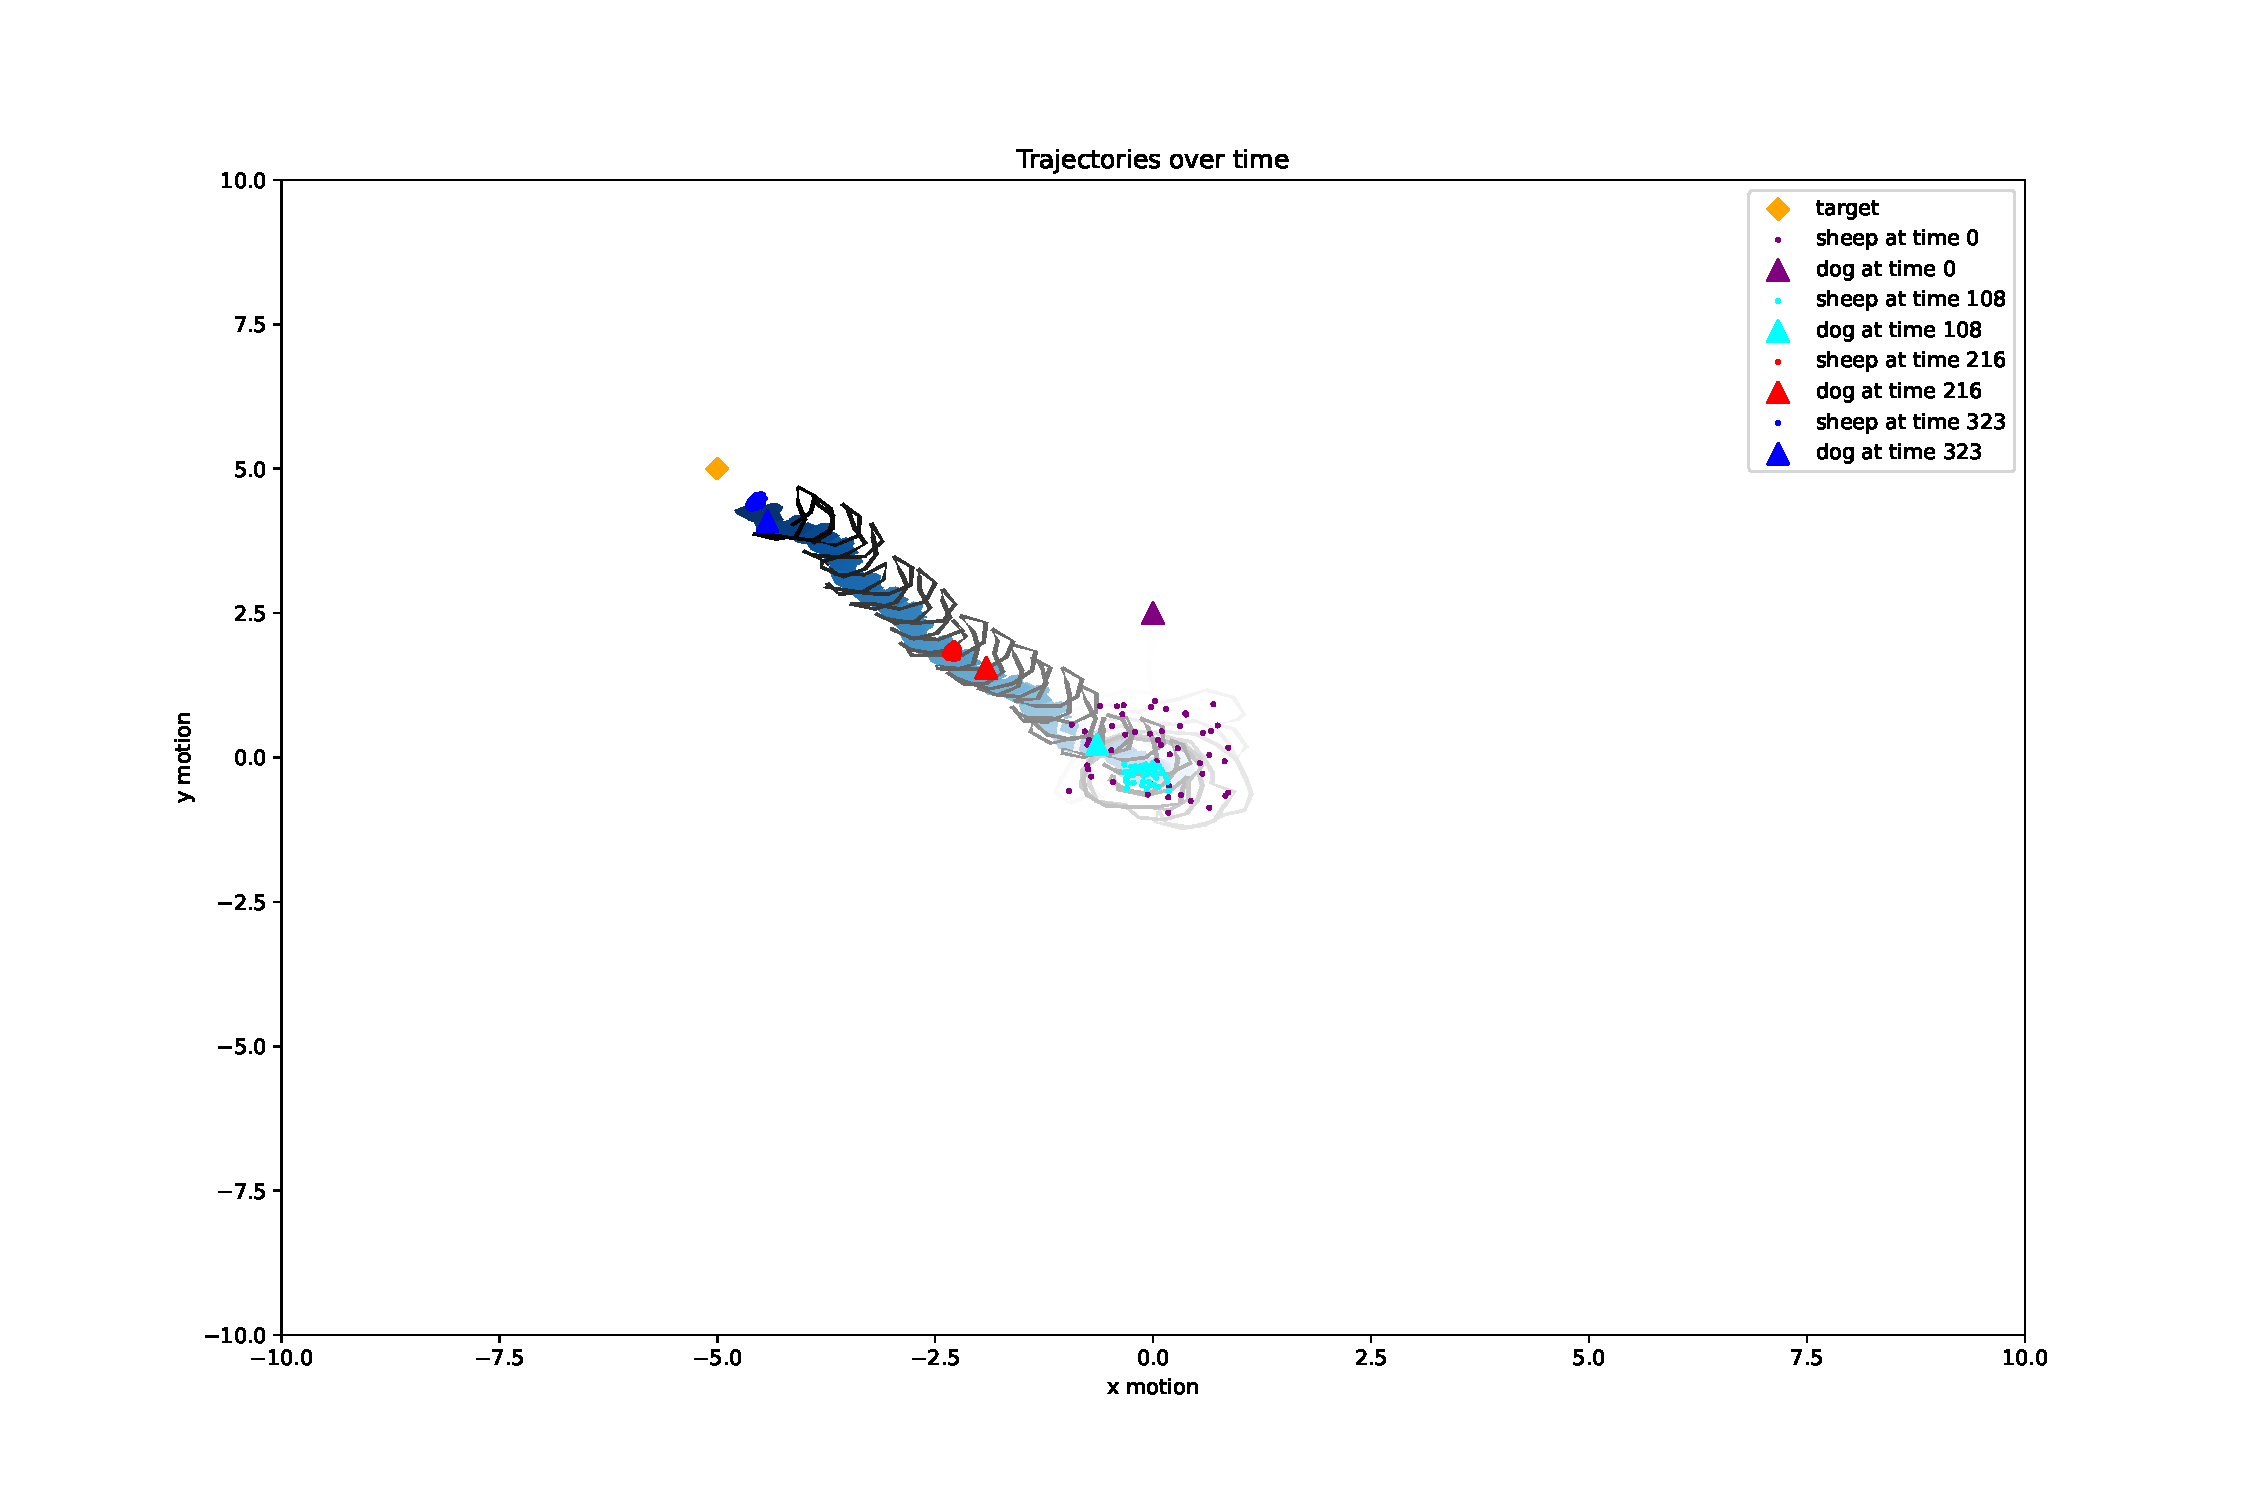
\includegraphics[width=\textwidth]{figures/droving.pdf}
%     \caption{}
%   \end{minipage}
%   \hfill
%   \begin{minipage}[b]{0.49\textwidth}
%     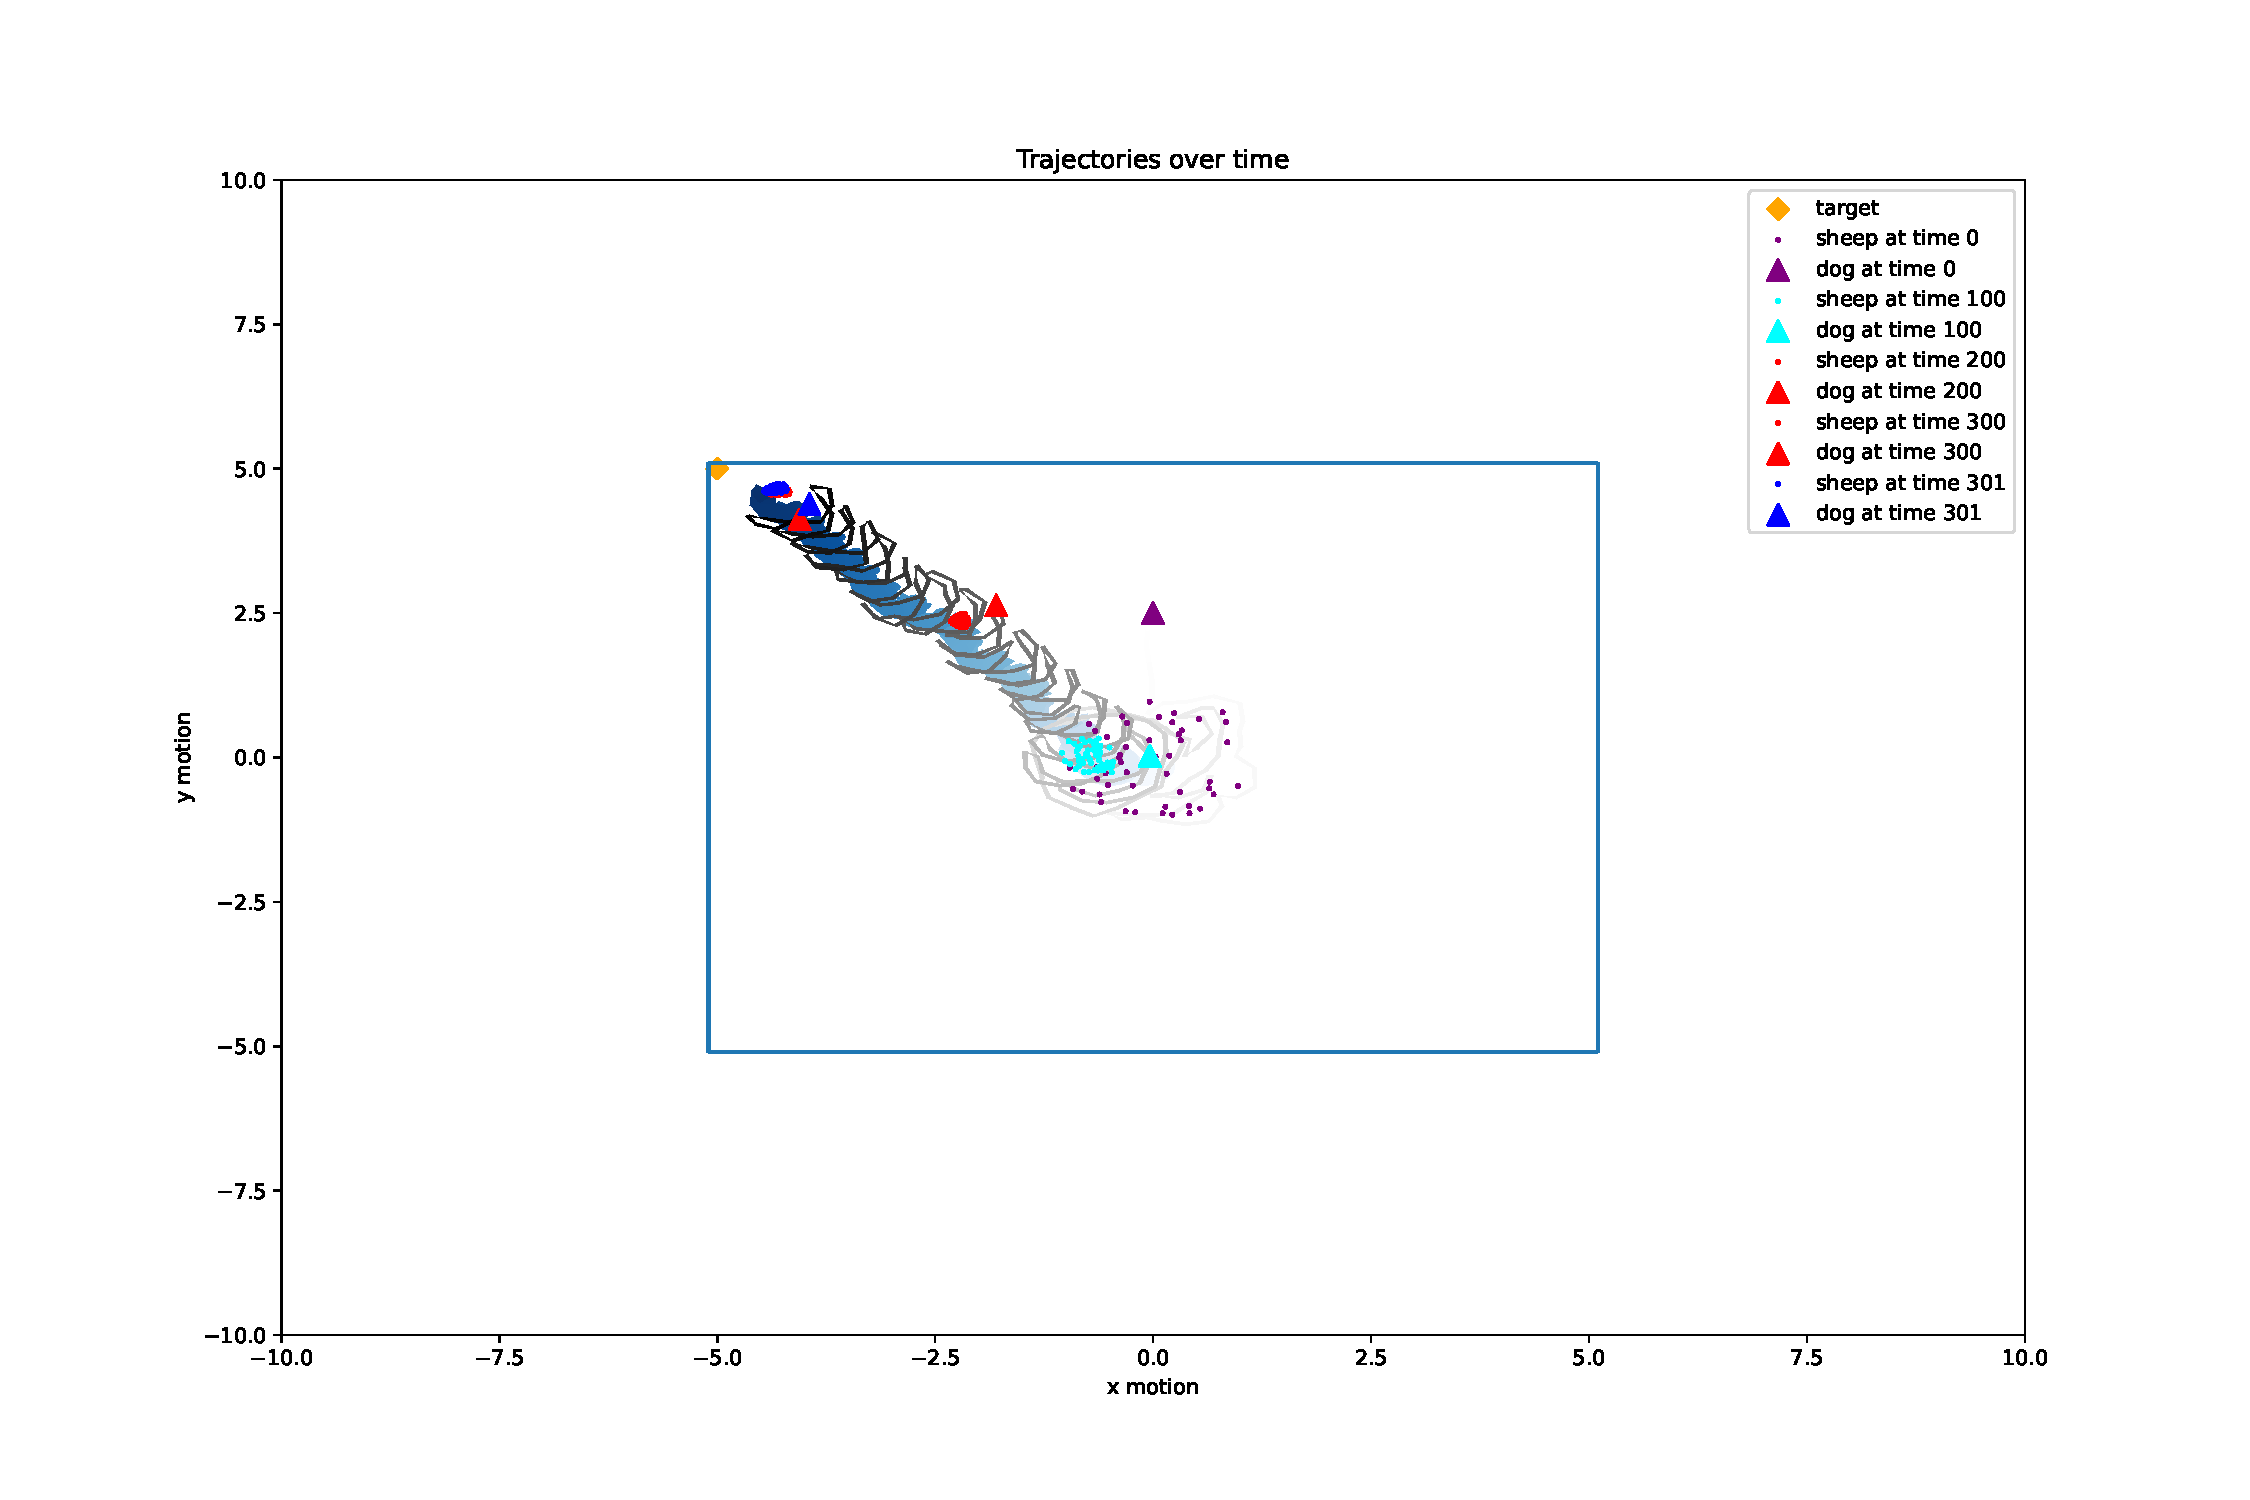
\includegraphics[width=\textwidth]{figures/droving-fence.pdf}
%     \caption{}
%   \end{minipage}
% \end{figure}

% \begin{figure}[!h]
%   \centering
%   \begin{minipage}[b]{0.49\textwidth}
%     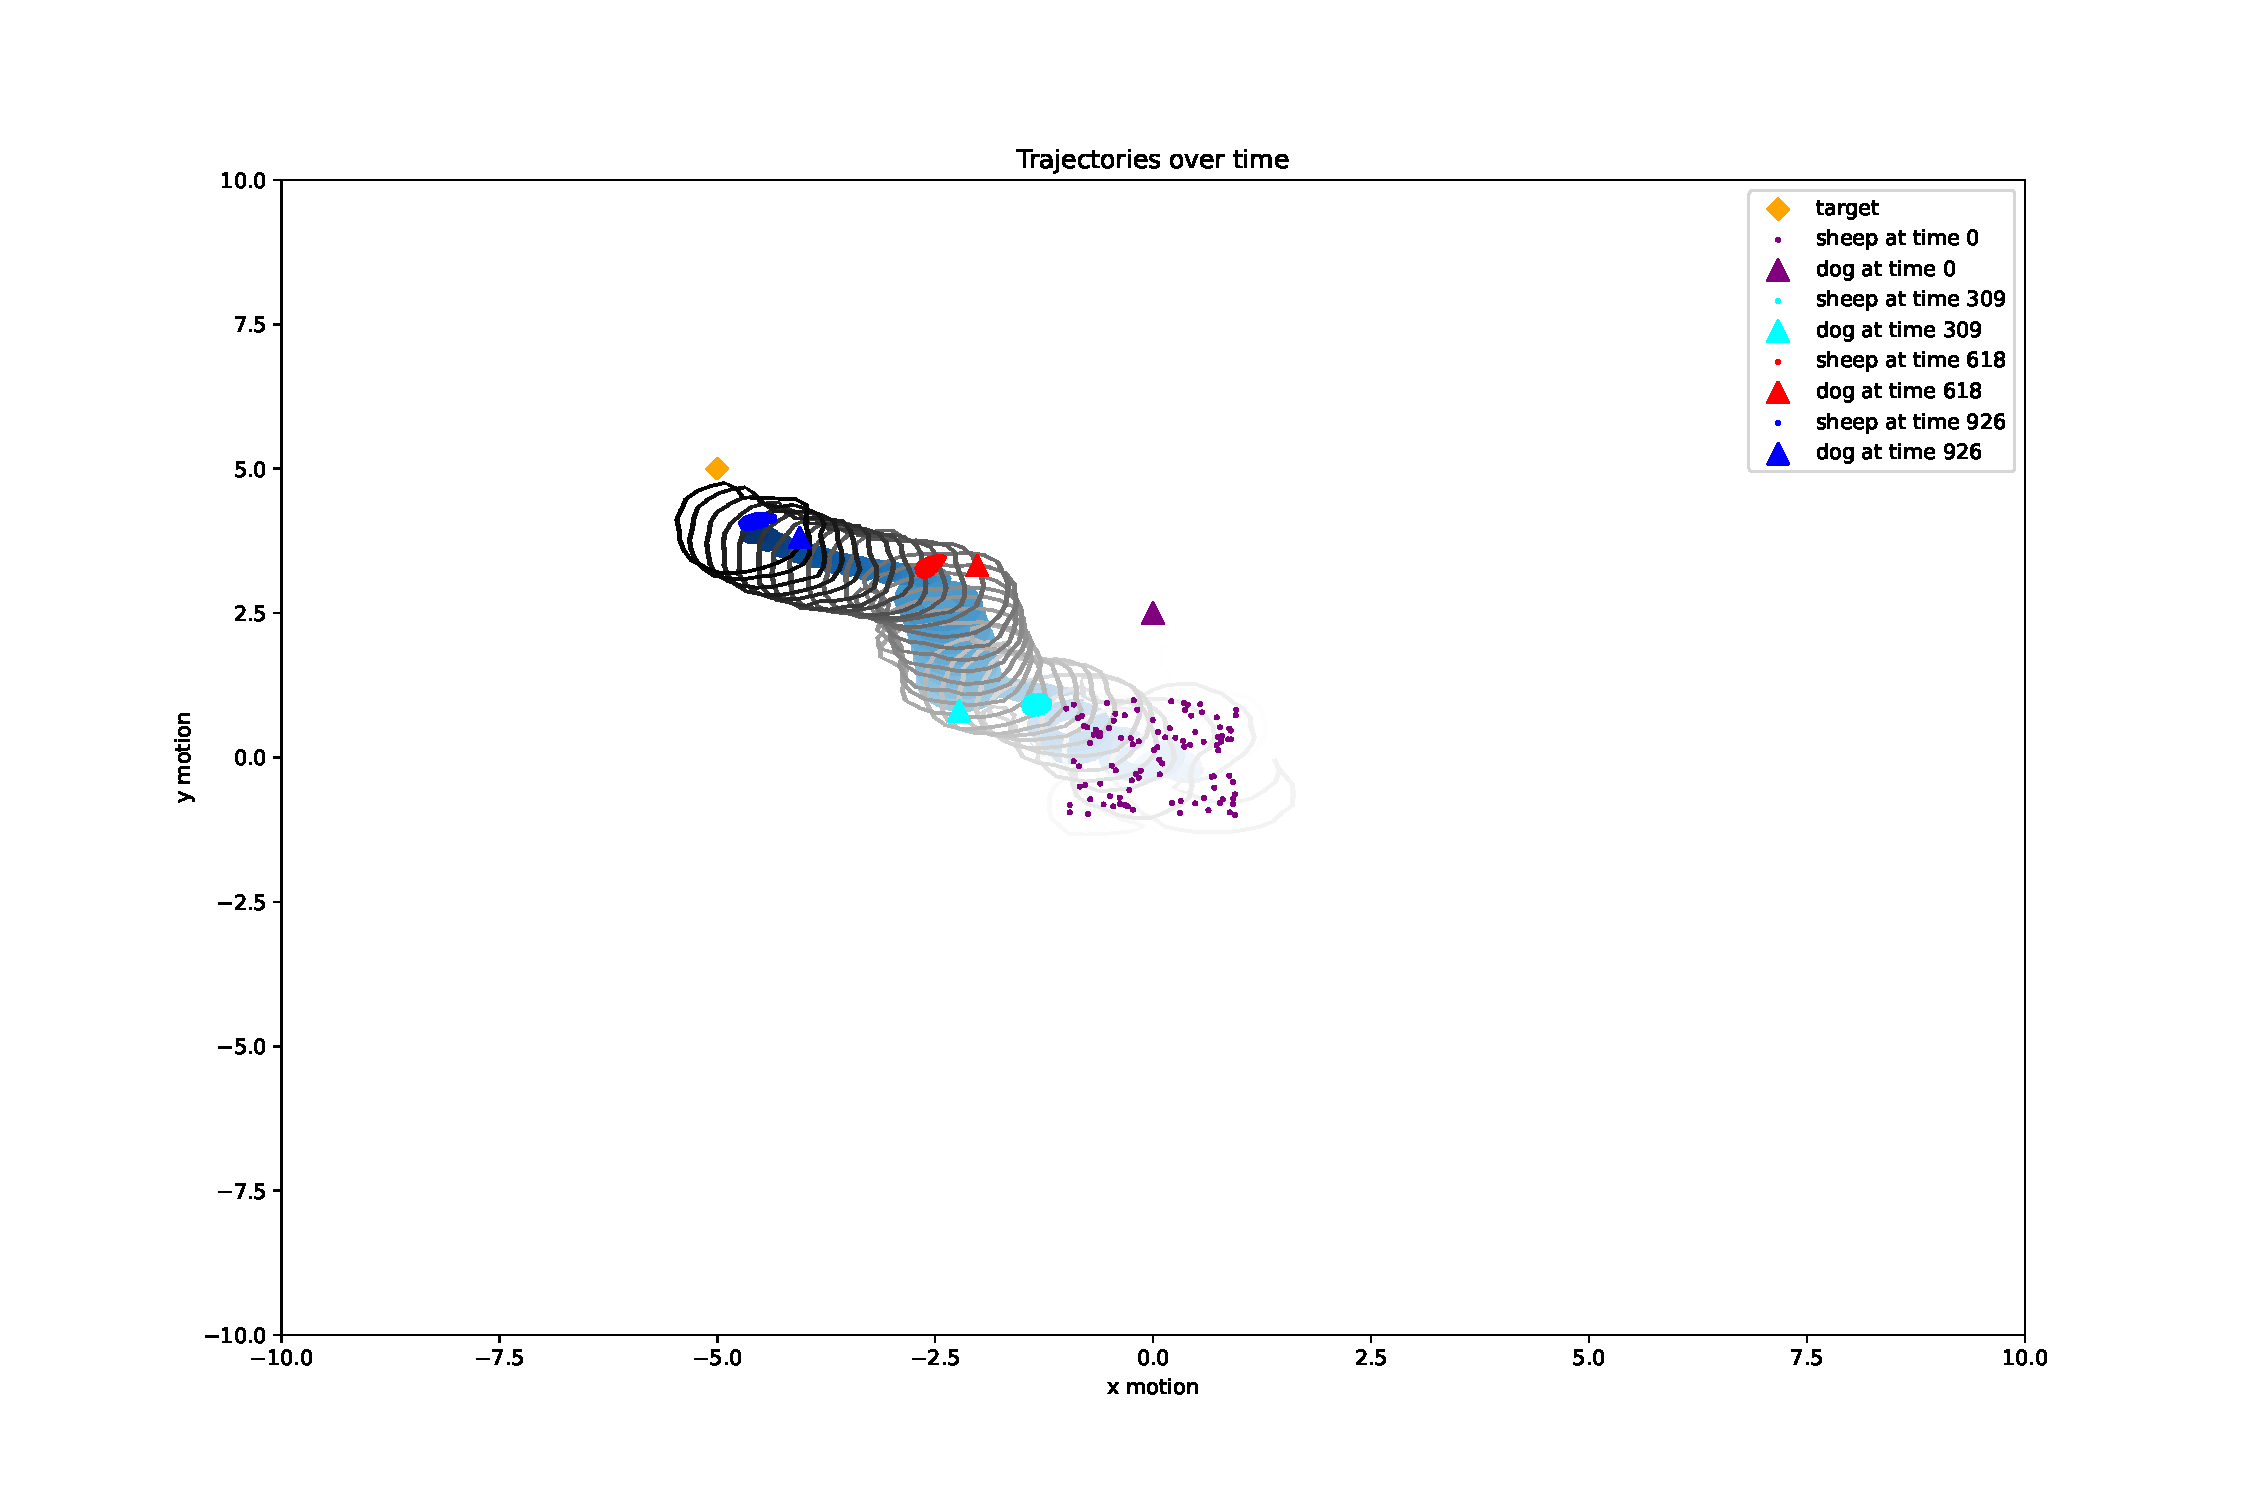
\includegraphics[width=\textwidth]{figures/mustering.pdf}
%     \caption{}
%   \end{minipage}
%   \hfill
%   \begin{minipage}[b]{0.49\textwidth}
%     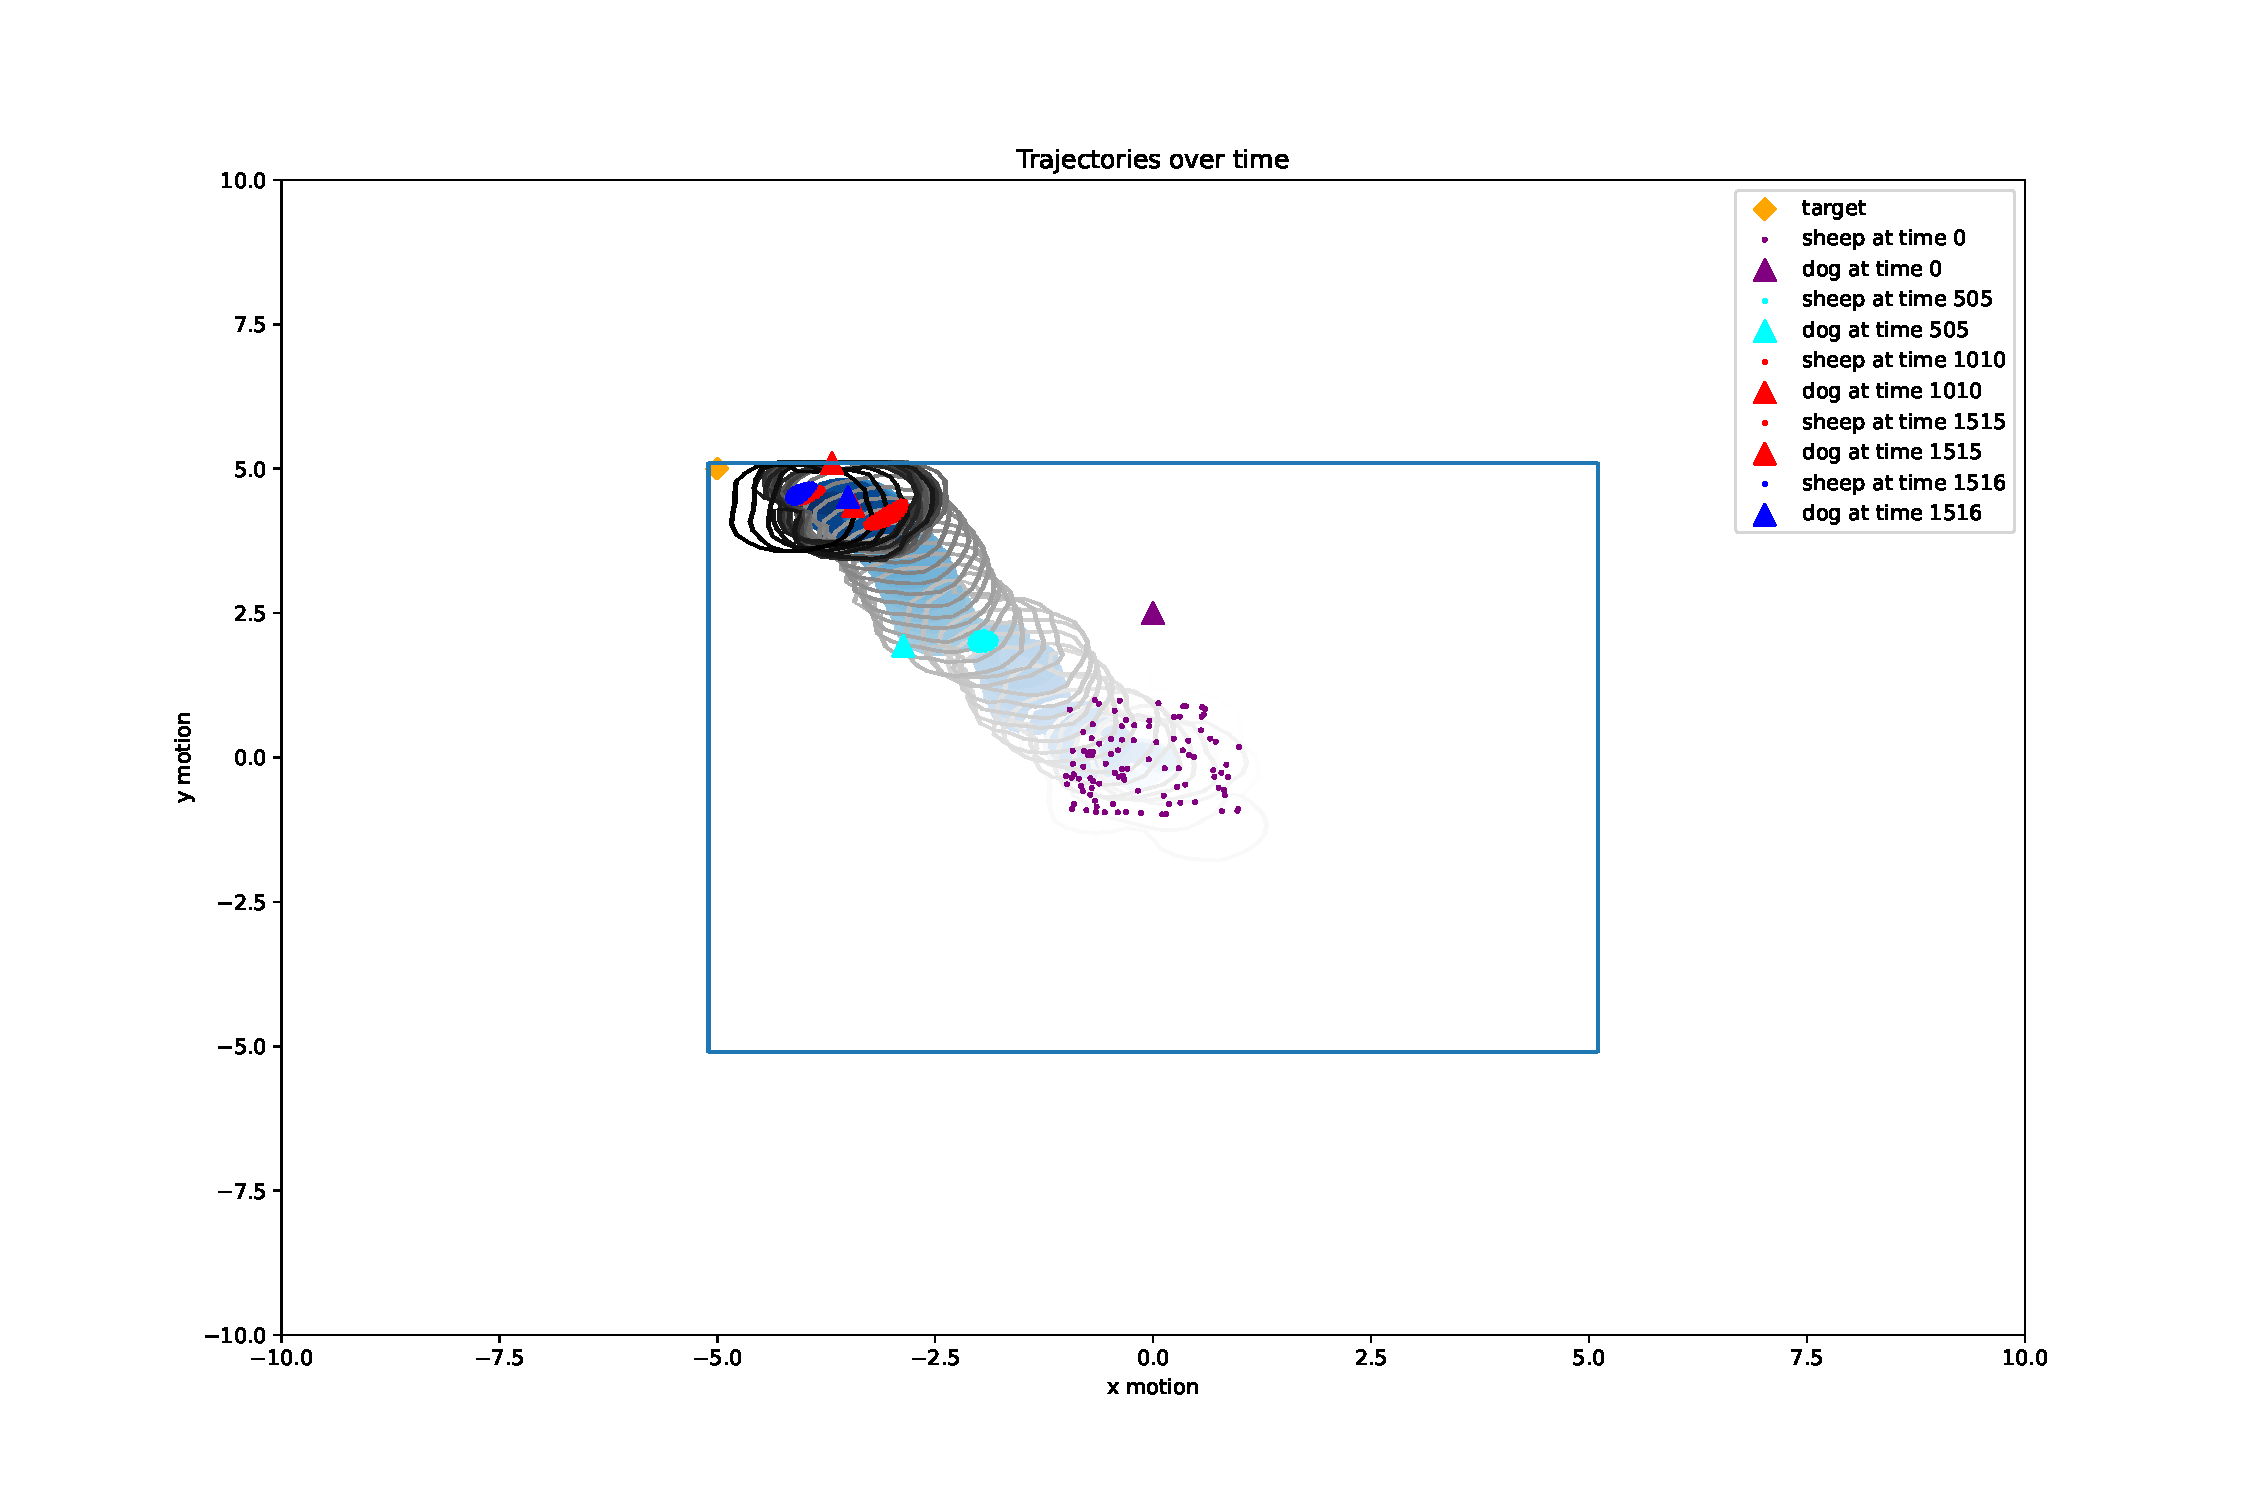
\includegraphics[width=\textwidth]{figures/mustering-fence.pdf}
%     \caption{}
%   \end{minipage}
% \end{figure}


\section*{Discussion}
\label{sec:discussion}
In this report we have described the overall topic and the current state of our project about optimal shepherding strategies. We have understood the ABM presented in the paper \textit{Optimal shepherding and transport of a flock} and plan to use it as starting point for our own investigation. We have already run the existing implementation of the ABM and identified the code files which are relevant for our project.

Our initial plan involved the idea of translating the original implementation from C++ to Python. We felt that Python, being a language we are more comfortable with, would facilitate modifying and adjusting the code. However, upon further examination and considering the feedback from fellow students, we have reconsidered this approach. We now believe that such a translation is not necessary, as we can reuse and extend the existing code with a manageable degree of effort. Additionally, the conversion to Python could potentially have a negative impact on the performance of the simulation.

For the kick-off, we did not yet have concrete ideas for extending our chosen paper. Now, as our comprehension of the ABM has improved, we have identified the scenario of having multiple shepherds as a a suitable extension of the paper's content. This scenario is highlighted as an open question for future study by the authors of our selected paper and was also proposed by fellow students.

Until the second report deadline, we will try to extend the ABM implementation such that it supports multiple shepherds. A possible goal for the final report is to investigate which optimal herding behaviors emerge in the case of more than one shepherd.


\section*{Conclusion and outlook}
\label{sec:conclusion}
In this project, we have built upon the agent-based shepherding model from the paper \textit{Optimal Shepherding and Transport of a Flock} \cite{ranganathan2022optimal} and extended it by introducing a surrounding fence and additional shepherds. Additionally, we have compared our approach to the existing agent-based shepherding model from the paper \textit{Simulating Single and Multiple
Sheepdogs Guidance of a Sheep Swarm} \cite{baxter2021simulating}.

Possible next steps include a more detailed analysis of our extensions. It would be interesting to study whether the three observed shepherding behaviours driving, droving, and mustering also arise for more than one shepherd and, if so, for which sets of parameters. Furthermore, one could extend the model even further, for example by introducing obstacles along the path from the herd to the target.

\acknow{
\textit{Franziska Weber} took care of the GitHub repository, researched existing models with multiple shepherds, wrote the description of the original model, analyzed the effect of introducing multiple shepherds, implemented the alternative agent-based shepherding algorithm and compared it to the optimization-based approach.
\textit{Kimberley Frings} corrected and initially executed the existing implementation, implemented the model extensions with a fence and multiple shepherds, composed all three reports and analyzed the effect of introducing a surrounding fence. \textit{Franz Muszarsky} created the presentation and the video. All three worked on understanding the implementation of the model and on the organization of the project.} 
\showacknow % Display the acknowledgments section

% \pnasbreak splits and balances the columns before the references.
% If you see unexpected formatting errors, try commenting out this line
% as it can run into problems with floats and footnotes on the final page.
%\pnasbreak

\begin{multicols}{2}
\section*{\bibname}
% Bibliography
\bibliography{bibliography}
\end{multicols}

\newpage

\section*{Appendix}
\label{sec:appendix}
\appendix
\begin{figure}[!h]
    \hspace*{-0.5cm}
    \includegraphics[width=0.85\textwidth]{"Third report/figures/driving_one_dog"}
    \caption{Trajectory plot for one shepherd in the driving scenario without a fence.  The colors of the agents indicate their orientation.}
    \label{fig:one-shepherd-no-fence}
\end{figure}

\begin{figure}[!h]
    \hspace*{-0.5cm}
    \includegraphics[width=0.85\textwidth]{"Third report/figures/driving_one_dog_fence"}
    \caption{Trajectory plot for one shepherd in the driving scenario with a fence.}
    \label{fig:one-shepherd-fence}
\end{figure}

\begin{figure}[!h]
    \hspace*{-0.5cm}
    \includegraphics[width=0.9\textwidth]{"Third report/figures/droving_one_dog"}
    \caption{Trajectory plot for one shepherd in the droving scenario.}
    \label{fig:single-shepherd}
\end{figure}

\begin{figure}[!h]
    \hspace*{-0.5cm}
    \includegraphics[width=0.9\textwidth]{"Third report/figures/droving_two_dogs"}
    \caption{Trajectory plot for two shepherds in the droving scenario.}
    \label{fig:two-shepherd}
\end{figure}

\end{document}








